\section{Versuchsaufbau}
Eine Schematische Zeichnung der DREAMS-Anlage ist in Abb. \ref{Auswertung_Bild_DREAMS} zu finden.
\begin{figure}[ht]
	\centering
    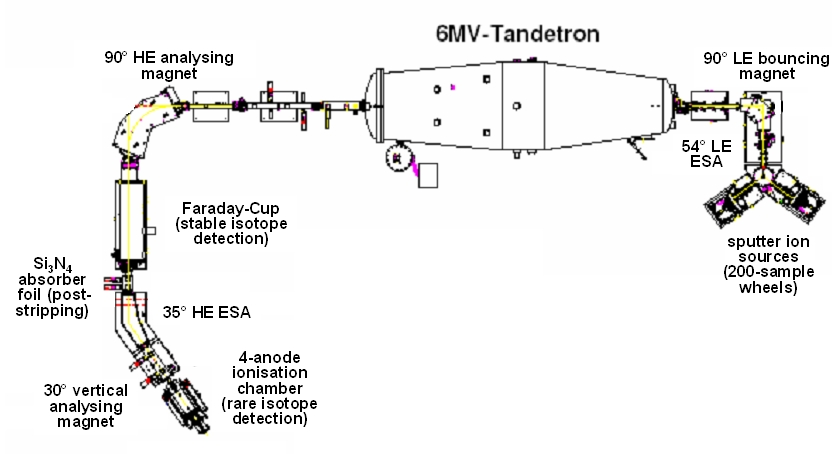
\includegraphics[width=0.85\textwidth]{Pictures/DREAMS.png}
	\caption{Schematik DREAMS \cite{Bild_DREAMS}}
	\label{Auswertung_Bild_DREAMS}
\end{figure}
Sie besteht aus folgenden Komponenten:
\begin{itemize}
    \item Sputter-Ionenquelle
    \item \ang{54} elektrostatischer Analysierer auf der Niederenergieseite
    \item \ang{90} Ablenkmagnet auf der Niederenergieseite
    \item \SI{6}{\mega\electronvolt} Tandem-Beschleuniger
    \item \ang{90} Ablenkmagnet auf der Hochenergieseite
    \item Faraday-Cups zur detektierung stabiler Isotope
    \item SiN Absorberfolie
    \item \ang{35} elektrostatischer Analysierer auf der Hochenergieseite
    \item \ang{30} vertikaler Analysemagnet
    \item Ionisationskammer mit 4 Anoden
\end{itemize} % weitere erklärungen?
